\documentclass[
../../EiKI_Summary.tex,
]
{subfiles}
    
\externaldocument[ext:]{../../EiKI_Summary.tex}
% Set Graphics Path, so pictures load correctly
\graphicspath{{../../}}

\begin{document}
\section{Bayesian Networks}
Bayesian Networks are a simple graphical notation for \defc{conditional independence} assertions, hence for \defc{compact specifications of full joint distributions}.

A Bayesian Network is \defc{directed, acyclic graph} with

\begin{itemize}
    \item \defc{Nodes:} One node per variable
    \item \defc{Edges:} A directed edge from node $N_i$ to node $N_j$ indicates that the corresponding variable $X_i$ has a direct influence on $X_j$
\end{itemize}

\defc{Set of random variables $\{X_1, \ldots, X_n\}$}

\begin{center}
    \defc{Directed Acyclic Graph (DAG)}

    \begin{tikzpicture}
        % Nodes
        \node[latent,fill=codepurple,text=white] (S) {S};
        \node[latent,fill=codepurple,text=white, above left=of S] (A) {A};
        \node[latent,fill=codepurple,text=white, above right=of S] (F) {F};
        \node[latent,fill=codepurple,text=white, below left=of S] (N) {N};
        \node[latent,fill=codepurple,text=white, below right=of S] (H) {H};

        % Edges
        \edge {S} {N, H};
        \edge {A} {S};
        \edge {F} {S};
    \end{tikzpicture}
\end{center}

\defc{Conditional Probability Distribution (CPD)}
\begin{itemize}
    \item Each randome variable $X_i$ in the network is associated with a CPD given its parents $(Pa(X_i))$
    \item \begin{smallmathbox*}
            $P(X_i | Pa(X_i))$
    \end{smallmathbox*}
    \item Each variable is probabilistically dependent on its parents
\end{itemize}

\defc{Joint Distribution:}

\begin{csmb*}
    $\displaystyle P(X_1, \ldots, X_n) = \prod_{i=1}^{n} P(X_i | Pa(X_i))$
\end{csmb*}

\defc{Local Markov Assumption:}\\
Each random variable $X_i$ is conditionally independent of its non-descendants, given its parents. 

\begin{csmb*}
    $X_i \bot \text{nonDescendants} | Pa(X_i)$
\end{csmb*}

\newpage
\subsection{Na\"ive Bayes }
A \defc{na\"ive Bayes} model assumes that all effects are independent given the cause:

\begin{csmb*}
    $\displaystyle P(\text{hypothesis}, \text{evidence}_1, \ldots, \text{evidence}_n) = P(\text{hypothesis}) \cdot \prod_{i=1}^{n} P(\text{evidence}_i | \text{hypothesis})$
\end{csmb*}

\begin{figure}[H]
    \centering
    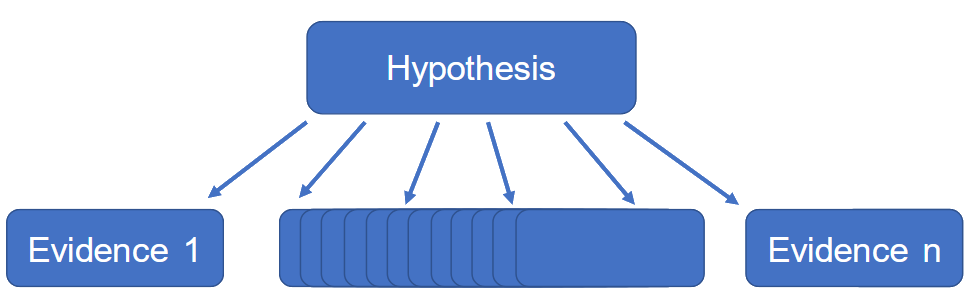
\includegraphics[width=0.8\textwidth]{Pics/09/NaiveBayesModel.png}
\end{figure}

\subsection{Inference in Bayesian Networks}

\defc{Query} P(X|e)

\defc{Definition of conditional probability:} $P(X|e) = \dfrac{P(X,e)}{P(e)}$

\defc{Up to normalization:} $P(X|e) \propto P(X,e)$

Can be rewritten as:

\begin{csmb*}
    $\displaystyle P(Y) = \underbrace{\sum_{X_i \notin Y}}_{\text{Marginalization}} \underbrace{\prod_{i=1}^{n} P(X_i | Pa(X_i))}_{\text{BN Semantics}}$
\end{csmb*}

\subsubsection{Variable Elimination}
Given a Bayesian Network and a query $P(X|e) / P(X,e)$.

Instantiate evidence e.

Choose an elimination order over the variables $X_1, \ldots, X_n$.

Initial factors of probability distribution comprised of: $f_1, \ldots, f_n$.

For i = 1 to n, if $X_i \notin \{X,E\}$:

Collect factors $f_1, \ldots, f_k$ that contain $X_i$.

Generate a new factor by eliminating $X_i$ from $f_1, \ldots, f_k$:

\begin{csmb*}
    $\displaystyle g = \sum_{X_i} \prod_{j=1}^{k} f_j$
\end{csmb*}

Remove all factors $f_1, \ldots, f_k$ and add new factor $g$ to the network. 

Normalize $P(X,e)$ to obtain $P(X|e)$.

\subsubsection*{Example}

\begin{center}
    \begin{tikzpicture}[
        every node/.style={latent,fill=codepurple,text=white,shape=rectangle, text width=60pt, align=center},
        ]
        % Nodes
        \node[] (V) {Visit to TB Country};
        \node[below left=of V] (T) {Tubercolosis};
        \node[below right=of T] (A) {Abnormality in Chest};
        \node[right=of V] (S) {Smoking};
        \node[below left=of S] (C) {Cancer};
        \node[below right=of C] (B) {Bronchitis};
        \node[below left=of B] (D) {Dyspnea};
        \node[below left=of A] (X) {X-Ray};

        % Edges
        \edge {V} {T};
        \edge {T} {A};
        \edge {A} {X, D};
        \edge {S} {C, B};
        \edge {C} {A};
        \edge {B} {D};
    \end{tikzpicture}
    \begin{tikzpicture}[
        every node/.style={latent,fill=codepurple,text=white, align=center},
        ]
        % Nodes
        \node[] (V) {V};
        \node[below left=of V] (T) {T};
        \node[below right=of T] (A) {A};
        \node[right=of V] (S) {S};
        \node[below left=of S] (C) {C};
        \node[below right=of C] (B) {B};
        \node[below left=of B] (D) {D};
        \node[below left=of A] (X) {X};

        % Edges
        \edge {V} {T};
        \edge {T} {A};
        \edge {A} {X, D};
        \edge {S} {C, B};
        \edge {C} {A};
        \edge {B} {D};
    \end{tikzpicture}
\end{center}

Assume we want to compute P(d), so we need to \defc{eliminate} v,s,t,c,a,b,x.

The \defc{probability distribution} is given as the product of multiple factors:

\begin{csmb*}
    $P(v,s,t,c,a,b,x,c) = P(v)P(s)P(t|v)P(c|s)P(b|s)P(a|c,l)P(x|a)P(d|a,b)$
\end{csmb*}

Lets choose the elimination order: v,s,x,t,c,a,b

From that we get:

\begin{csmb*}
    $\begin{array}{c|c r l}
        && P(v,s,x,t,c,a,b,d) &= P(v)P(s)P(t|v)P(c|s)P(b|s)P(a|c,l)P(x|a)P(d|a,b)\\
        v&\Rightarrow & P(s,x,t,c,a,b,d) &= \defco{f_v(t)}P(s)P(c|s)P(b|s)P(a|c,l)P(x|a)P(d|a,b)\\
        s&\Rightarrow & P(x,t,c,a,b,d) &= f_v(t)\defco{f_s(b,c)}P(a|t,c)P(x|a)P(d|a,b)\\
        x&\Rightarrow & P(t,c,a,b,d) &= f_v(t)f_s(b,c)\defco{f_x(a)}P(a|t,c)P(d|a,b)\\
        t&\Rightarrow & P(c,a,b,d) &= f_s(b,c)f_x(a)\defco{f_t(a,c)}P(d|a,b)\\
        c&\Rightarrow & P(a,b,d) &= f_x(a)\defco{f_c(a,b)}P(d|a,b)\\
        a&\Rightarrow & P(b,d) &= \defco{f_a(b,d)}\\
        b&\Rightarrow & P(d) &= \defco{f_b(d)}\\
    \end{array}$
\end{csmb*}

\hrule

This unfortunately is not efficient. 

\begin{center}
    \begin{smalldefbox}
        [Theorem]
        Inference (even approximate in Bayesion networks is NP-Hard)
    \end{smalldefbox}
\end{center}

\subsubsection{Approximate Inference by Stochastic Sampling}
\textbf{Basic Idea:}
\begin{enumerate}
    \item Draw \defc{$N$} samples from a sampling distribution \defc{$S$}
    \item Compute an approximate posterior probability \defc{$\hat{P}$}
    \item Show this converges to the true probability \defc{$P$}
\end{enumerate}

\subsubsection*{Draw samples}
\textbf{Given:}
\begin{itemize}
    \item Random Variable \defc{$X | D(X) = \{0,1\}$}
    \item $P(X)$ = \{0.3, 0.7\} (P(X=0) = 0.3, P(X=1) = 0.7)
\end{itemize}

\textbf{Sample X = P(X)}
\begin{itemize}
    \item Get a random number $r \in [0,1]$
    \item If $r < 0.3$ then $X = 0$
    \item Else $X = 1$ 
\end{itemize}

Can be generalized to any domain size.

\subsubsection*{Sampling from ''Empty Network''}
Ergo, \defc{generating samples from a network that has no evidence associated with it.}

\textbf{Basic Idea:}
\begin{itemize}
    \item Sample a value for each variable in topological (in respect to dependencies) order
    \item Using the specified conditional probabilities
\end{itemize}

\begin{codebox*}
    \begin{algorithm}[H]
        \SetKwFunction{priorsample}{prior\_sample}

        \tcp{belief network specifies joint distribution $P(X_1, \ldots, X_n)$}
        \Fn{\priorsample{belief\_network} $\rightarrow$ event sampled from belief network}{
            x = event with n elements\;
            \For{i = 1 \KwTo n}{
                $x_i$ = random sample from $P(X_i | Pa(X_i))$ given the values of $Pa(X_i)$ in x\;
            }
            \KwRet x
        }
    \end{algorithm}
\end{codebox*}

\textbf{Example:}\\
\begin{figure}[h]
    \centering
    \begin{tikzpicture}
        
        % Nodes
        \node[latent,shape=ellipse,text width=40pt,align=center] (C) {Cloudy};
        \node[latent,shape=ellipse,text width=40pt,align=center, below left=of C] (S) {Sprinkler};
        \node[latent,shape=ellipse,text width=40pt,align=center, below right=of C] (R) {Rain};
        \node[latent,shape=ellipse,text width=40pt,align=center, below right =of S] (W) {Wet Grass};

        \node[above =10pt of C] {
            \begin{tabular}{|c|}
            \hline
            P(C) \\
            \hline
            0.50 \\
            \hline
        \end{tabular}
        };
        \node[left =10pt of S] {
            \begin{tabular}{|c|c|}
                \hline
                C & P(S|C) \\
                \hline
                T & 0.10 \\
                F & 0.50 \\
                \hline
            \end{tabular}
        };
        \node[right =10pt of R] {
            \begin{tabular}{|c|c|}
                \hline
                C & P(R|C) \\
                \hline
                T & 0.80 \\
                F & 0.20 \\
                \hline
            \end{tabular}
        };
        \node[below =10pt of W] {
            \begin{tabular}{|c|c|c|c|}
                \hline
                S & R & P(W|S,R) \\
                \hline
                T & T & 0.99 \\
                T & F & 0.90 \\
                F & T & 0.90 \\
                F & F & 0.01 \\
                \hline
            \end{tabular}
        };
        % Edges
        \edge {C} {S};
        \edge {C} {R};
        \edge {S} {W};
        \edge {R} {W};
    \end{tikzpicture}
    \caption{Bayesian Network for Weather and Wet Grass}
\end{figure}

\subsubsection*{Probability Estimation using Sampling}
Calculating a probability estimation:
\begin{itemize}
    \item Sample many points using the algorithm above
    \item Count how often each possible combination $x_1, \ldots, x_n$ occurs
    \item Estimate the probability by the observed percentages \\
    \begin{smallmathbox*}
        $\hat{P}(x_1, \ldots, x_n) = N_{PS}(x_1, \ldots, x_n) / \text{number of samples}$
    \end{smallmathbox*}
\end{itemize}

This converges towards the joint probability function.

\subsubsection*{Markov Chain Monte Carlo (MCMC) Sampling}
\begin{codebox*}
    \begin{algorithm}[H]
        \SetKwFunction{mcmcask}{mcmc\_ask}
        \SetKwFunction{normalize}{normalize}

        \Fn{\mcmcask{X,e,belief\_network, num\_samples} $\rightarrow$ estimate of $P(X|e)$}{
            count\_X = [] \tcp{number of times each X occurs, initially 0 for all}
            Z = [non-evidence variables] \tcp{list of non-evidence variables}
            x = e \tcp{current state of the network, initially e}

            initialize non-evidence values in x with random values\;

            \tcp{Gibbs sampling}
            \For{j=1 \KwTo num\_samples}{
                \ForEach{$Z_i \in Z$}{
                    x[$Z_i$] = sample from $P(Z_i | \text{markov\_blanket}(Z_i))$
                }
                count\_X[x] += 1 \tcp{x is the value of X in x}
            }
            \KwRet \normalize{count\_X}
        }
    \end{algorithm}
\end{codebox*}

More samples result in better approximates.

\begin{defbox}
    [Markov Blanket]
    A Markov Blanket is a set of variables that are conditionally independent of a variable given all other variables in the network. It consists of \defc{parents (direct causes), children (direct effects) and childrens parents (co-causes)}.
    Alternatively: A markov blanket includes all variables that \defc{directly influence} or \defc{are influenced} by a variable $X$. Everything outside of the markov blanket is irrelevant to $X$. This makes it easier to compute probabilities.

    \begin{csmb*}
        $P(X | U_1, \ldots, U_m, Y_1, \ldots, Y_n, Z_{1j}, \ldots, Z_{nj}) = P(X | \text{all variables})$
    \end{csmb*}

    \begin{center}
        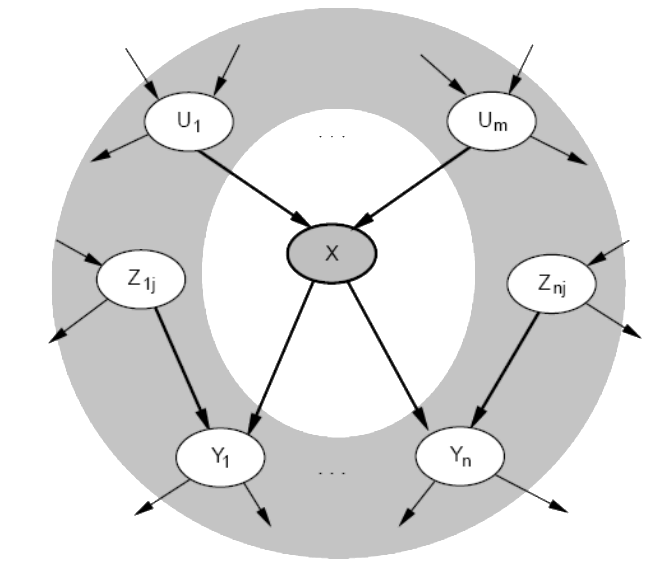
\includegraphics[width=0.4\textwidth]{Pics/09/MarkovBlanket.png}
    \end{center}

\end{defbox}

\begin{defbox}
    [Gibbs Sampling]
    Basic Idea:
    \begin{enumerate}
        \item \defc{Initialize} all variables with random values
        \item \defc{Iterate through each variable}, updating it based on Markov Blanket
        \item \defc{Repeat} until samples converge to the true distribution
    \end{enumerate}

    Gibbs Sampling utilized Markov Blankets by reducing the number of variables that need to be considered at each step.
\end{defbox}

\textbf{Example:}\\
Estimate $P(\text{Rain}|\text{Sprinkler = true, WetGrass = True})$

\begin{enumerate}
    \item Sample Cloudy or Rain given its Markov Blanket, repeat n times
    \item Count number of times Rain is true and false in the samples 
\end{enumerate}

E.g. sample 100 states and count 31 times Rain and 69 times not Rain.

\begin{csmb*}
    $P(\text{Rain}|\text{Sprinkler = true, WetGrass = True}) =$ \texttt{Normalize$<31,69>$} = $<0.31, 0.69>$
\end{csmb*}

\begin{defbox}
    [Theorem]
    Chain approaches stationary distribution:

    Long-run fraction of time spent in each sate is exactly proprotional to posterior probability.
\end{defbox}
\end{document}